\chapter{Tests}

This chapter includes test descriptions and results to validate the design against the requirements. First, the two directional antennas are tested to find their gain and ensure, that the transmitter and receiver have their maximum gain at the same frequency. Finally, the full test of the beam steering and transmitter locator is tested with the transmitter fixed at a known location in the test area.

\section{Test of Gain in Frequency Spectrum} 
The aim of this test is to test both directive antennas in a frequency spectrum to ensure they operate at the same frequency.


\section{Test of Radiation Pattern}
The aim of this test is to know the directiveness of the two directional antennas.


\section{Accept Test}
The aim of this test is to test the full function of the developed product. The test must show that the receiver antenna on the turntable is able to scan the test area and measure the received power at fixed angles, before selection the location with the maximum received power and focusing its beam on that location.

\subsubsection{Equipment}
To perform the test, the following equipment is needed:

\begin{itemize}
    \item HEAD Acoustics Remote-operated Turntable, model HRT I 6498, with \SI{24}{\volt} \SI{60}{W} power supply
    \item D-sub 9-pin to USB-A cable
    \item PC with one USB-A port and XX port
    \item VNA ???
    \item VNA cable ???
    \item Two \SI{50}{\ohm} directional antennas with XX frenquecy
    \item power supplies to the antennas ????
\end{itemize}

Moreover, the test must be performed in a controlled environment, where the temperature is not below \SI{0}{\celsius} or above \SI{50}{\celsius} with a relative humidity in the range \SI{20}{\percent} - \SI{80}{\percent}~\cite{hrt_i_data_sheet}.
\todo{add VNA environmental conditions}

\subsubsection{Test Execution}
The following steps outline how to perform the test:

\begin{enumerate}
    \item Do this. Refer to figure \ref{fig:experiment-setup} to visualise the setup.
\end{enumerate}

\begin{figure}[h]
    \centering
    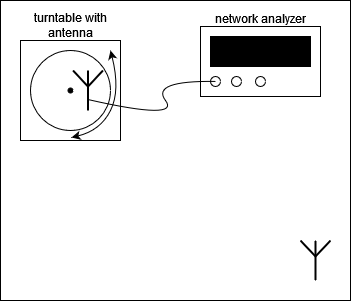
\includegraphics[width=0.5\textwidth]{figures/experiment-setup.png}
    \caption{Setup for test of functionality of beam steering device.} \label{fig:experiment-setup}
\end{figure}